\scanpage{170}
Énoncés plausibles (sur préschéma excellent de dim finie).
\diagram{$\unsure{\underline{D}|D}_X\left\{\begin{array}{l}
\unsure{\underline{D}|D}_c(X)^o\simeq\unsure{\underline{D}|D}_c(X)\\
\unsure{\underline{D}|D}_c^-(X)^o\xrightarrow{\sim}\unsure{\underline{D}|D}_c^+(X)\\
\unsure{\underline{D}|D}_c^+(X)^o\simeq\unsure{\underline{D}|D}_c^-(X)\\
\unsure{\underline{D}|D}_c^b(X)\simeq\unsure{\underline{D}|D}_c^b(X)
\end{array}\right.$}

$F_\bullet\in\operatorname{Ob}\unsure{\underline{D}|D}_c^-(X)$, \inserted{$G^{\bullet}=\unsure{\underline{D}|D}_X(F_\bullet)\in\operatorname{Ob}\unsure{\underline{D}|D}_c^+(X)$} je dis que
\[
(1)\qquad F_\bullet\text{ de Tor-dim finie}\Longleftrightarrow G^{\bullet}\text{ de pseudo dim. inj. finie}
\]
\margin{(**)}
\margin{\diagram{\begin{tikzcd}[ampersand replacement=\&,row sep=small]
\begin{gathered}\relax
[\text{i.e. }\inserted{\exists N\text{ tel que }}\text{pour tt }\deleted{\unsure{G_P}}P\deleted{\in\operatorname{Ob}\unsure{\underline{D}|D}_c}\inserted{\text{faisceau}}\\
\text{constructible, }\operatorname{Ext}^i(P,G^{\bullet})=0\\
\text{pour }i>N]
\end{gathered}\arrow[d,leftrightarrow]\\
\text{fibres géom. }G^{\bullet}_{\bar{x}}\text{ est de dim. inj. finie}\\
\text{(pour les }A\text{-Modules)}
\end{tikzcd}}}

\figure{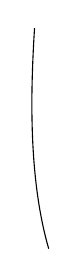
\begin{tikzpicture}[x=1cm,y=1cm]
\draw (0,0)..controls(-.05,-.8) and (-.08,-1.9)..(.18,-2.8);
\end{tikzpicture}}
\uline{N.B.} Si $X$ de dim abs. finie \unsure{on a} pour $G^{\bullet}$ donné ; $G^{\bullet}$ pseudo-dim. inj. finie $\Longleftrightarrow G^{\bullet}$ de dim. injective finie

Dém. de (1). L'implication $\longrightarrow$ formelle, en utilisant que $R_X^{\bullet}$ est de pseudo-dim. injective finie, et
\[
\mathbb{R}\mathcal{H}om^{\bullet}(P_\bullet,\unsure{\underline{D}|D}_X(F_\bullet))
=\mathbb{R}\mathcal{H}om^{\bullet}(P_\bullet,\mathbb{R}\mathcal{H}om^{\bullet}(F_\bullet,R_X^{\bullet}))
\simeq\mathbb{R}\mathcal{H}om^{\bullet}(P_\bullet\overset{\mathbb L}{\otimes}F_\bullet,R_X^{\bullet})
\]
Pour l'implication inverse, utiliser la bidualité pour $F_\bullet\overset{\mathbb L}{\otimes}P$ ----

\uline{NB.} Si les fibres géom $A_{\bar{x}}$ sont Gorenstein, alors en admettant l'équivalence (**), on voit que si $F_\bullet\in\operatorname{Ob}\unsure{\underline{D}|D}_c(X)$ Tor-dim finie $\Longleftrightarrow$ pseudo-dim inj. finie, et $\unsure{\underline{D}|D}_X$ induit une anti-autoequivalence dans la catégorie desdits complexes ...
\margin{169}
